\chapter{Gradient and categorical aspects of wordlikeness judgements}
\label{gradience}

\citet{Halle1962} and \citet{Chomsky1965} observe that speakers internalize generalizations about possible and impossible words in their language. \citeauthor{Chomsky1965} illustrate this knowledge with two nonce words \emph{blick} [blɪk] and \emph{bnick} [bnɪk]; whereas \emph{blick} is unattested, but possible word of English, 
speakers immediately recognize \emph{bnick} to be ill-formed, an impossible word of the language.

The classic account of this contrast is as follows. Segments must be assigned to prosodic structures like the syllable, or undergo phonological repair (e.g., \citealt{Hooper1973}:10f., \citealt{Ito1989a}, \citealt{Noske1992}). In English, [bl] is a permissible onset, but unlike some languages (e.g., Moroccan Arabic \emph{bni} `building', \emph{bnat} `daughters', \emph{bniqa} `closet'), [bn] is not. \citet[][19f.]{Wolf2009} suggest, for instance, that an underlying /bnɪk/ would be realized as [nɪk]; it is also possible to imagine resolution by prothesis---[əbnɪk]---or anapytxis---[bənɪk], and indeed \citet{Davidson2006b} finds that English speakers produce these repairs when attempting to mimic foreign pronunciations of obstruent-nasal onsets.

Many linguists view this account as overly simpliest, for, as \citeauthor{Shademan2006} argues, it draws a categorical boundary between the possible and impossible which fails to match the granularity at which speakers may report wordlikeness intuitions.

\begin{quote}
A defect of current grammatical acounts of phonotactics is that they render simple up-or-down decisions concerning well-formedness and cannot account for gradient judgements. But when judgements are elicited in a controlled fashion from speakers, they always emerge as gradient, including all intermediate values. \citep[][371]{Shademan2006} 
\end{quote}

This chapter focuses on the hypothesis that speakers' knowledge of wordlikeness is gradient. \S\ref{gradhyp} places this debate in a historical perspective, and argues that the naïve but widely accepted form of this hypothesis fails the test of falsifiability. In \S\ref{2evaluation}, a revision of this hypothesis is subjected to an quantitative evaluation and is found wanting.

[Explain that there's not going to be any issue of, e.g., heterovoiced obstruents, that stuff is all in chap. 4]

\section{The gradience hypothesis} \label{gradhyp}

%In this section, the gradience hypothesis is reviewed from historical and scientific perspectives. 

\subsection{A brief history of the gradience hypothesis} \label{history}

\citet{Chomsky1965} were not the first to consider contrasts between possible and impossible words. Their primary contribution to this question, is, essentially, mentalism: they recognize that naïve speakers effortlessly acquire language-specific wordlikeness generalizations and can report them with ease. But the nature of these contrasts were also considered by structuralists. In an early study, \citet{Fischer-Jorgensen1952} proposes that possible and impossible words represent endpoints on a continuum, and that no non-arbitrary line can be drawn between them. While it would anachronistic to assign this a mentalistic interpretation, this appears to be the earliest proposal that wordlikeness contrasts are in some sense gradient. 

\subsubsection{Early generative grammar}

Gradience is also discussed in the earliest work in generative syntax. \citet[][132]{LSLT} writes that ``there is little doubt that speakers can fairly consistently order new utterances, never previously heard, with respect to their degree of `belongingness' to the language''. \citet{ASPECTS} proposes to link different degrees of ungrammaticality to different kinds of syntactic violations. Unlike \citeauthor{Fischer-Jorgensen1952}, there is for \citeauthor{LSLT} a hard-and-fast boundary between the grammatical and ungrammatical, only the latter showing any gradience. For \citeauthor{LSLT}, grammatical utterances are all equally grammatical, but ungrammatical utterances may be deviant in their their own ways \citep[][61]{Schutze1996}.

However, most of the early literature on wordlikeness concerns apparently categorical contrasts the possible and impossible. \citet[][31]{Vogt1954} recognizes that the taxonomic phoneme is insufficient to account for many wordlikeness contrasts. Generalizing somewhat from \citeauthor{Vogt1954}'s discussion, allophony may account for the absence of certain phone sequences, but it does not provide a suitable explanation for the absence of initial [bn] in English, nor does it make correct predictions about the surface realization of an underlying initial /bn/. \citeauthor{Vogt1954} concludes that additional grammatical machinery will be needed to account for possible and impossible words. \citet{Halle1962} and \citet{Stanley1967} propose to derive wordlikeness effects from morphophonemic redundancy rules acting on underlying representations. The discussion of \emph{bnick} by \citet[][101]{Chomsky1965} is a good example of this type of analysis. They correctly observe that before a word-initial stop, a English consonant must be liquid. A side effect of a redundancy rule which specifies a consonant in this position as [$+$\textsc{Liquid}] precludes the derivation of \emph{bnick}.\footnote{This is not the only redundancy that might be used to rule out \emph{bnick}; for instance, the only word-initial obstruent that may follow a nasal in English is /s/.}

\subsubsection{\emph{The sound pattern of English}}

In \emph{The sound pattern of English} (SPE), \citet{SPE} extend this model of wordlikeness to account for 

[Explain the SPE model]

\subsubsection{Autosegmental phonology and beyond}

The \emph{SPE} model was not widely adopted, and research on wordlikeness turned to other principles. Syllabification plays no role in \emph{SPE} theory, though the syllable is found in many earlier studies (see \citealp{Goldsmith2011b}). \citet{Hooper1973} and \citet{Kahn1976} argue that wordlikeness generalizations argue for the need for syllabification as part of the phonological computation. This classic syllabification-based model is further enriched by the autosegmental theory of the syllable \citep{McCarthy1979b}, which envisions the syllable as an articulated tree structure \citep[as envisioned by][]{Pike1947a}, and the theory of prosodic licensing \citep{Ito1989a}, in which syllabification triggers phonological repairs.

\subsection{A naïve gradience axiom}

Recent critiques of this syllabification-based model focus on the existence of intermediate wordlikeness ratings (see also \citealt{Coleman1997}, \citealt{Anttila2008}). 

\begin{quote}
In the particular domain of phonotactics gradient intuitions are pervasive: they have been found in every experiment that allowed participants to rate forms on a scale.
\citep[][382]{Hayes2008a}

When native speakers are asked to judge made-up (nonce) words, their intuitions are rarely all-or-nothing. In the usual case, novel items fall along a gradient cline of acceptability. \citep[][9]{Albright2009a}
\end{quote}

The observation itself cannot be questioned, but \citeauthor{Hayes2008a} and \citeauthor{Albright2009a} do not explicitly state why this data is relevant to the construction of models of wordlikeness. The following seems the most likely: \citeauthor{Hayes2008a} and \citeauthor{Albright2009a} believe this proves that wordlikeness, as an internal state, is gradient simply because subjects make use of intermediate degrees of wordlikeness in judgement tasks. This proposition, generalized below, is ``naïve'' not because it lacks sophistication, but because it is rooted in a belief in naïve realism, a philosophy which holds that perception provides a relatively direct picture of the nature of the world, and an influential view in the cognitive sciences (see \citealt{Fodor1981a} for a critique).

\begin{unlabeledexample}
\textsc{Naïve Gradience Proposition}: If graded judgements of a concept or mental state use intermediate ratings, that concept or mental state is gradient
\end{unlabeledexample}

This proposition is an indicative conditional. While the antecedent of this condition, the presence or absence of intermediate ratings in a graded judgement task, is readily observable, it has no bearing on the truth or falsity of the conditional proposition. However, whereas a false consequent (e.g., an all-or-nothing concept) would potentially falsify the proposition, the consequent, a mental state, cannot be directly observed. If this is the case, then both the proposition and the consequent (the proposition that wordlikeness is itself gradient) fail the test of falsification, placing it beyond the reach of scientific inquiry.

\citet{Armstrong1983} cut the Gordian knot by asserting the possibility of observing a false consequent; they find the existence of all-or-nothing concepts like ``odd number'' or (more controversially) ``female'' to be apparent.

\begin{quote}
Are there definitional concepts? Of course. For example. consider the concept \emph{odd number}. This seems to have a clear definition, a precise description\ldots{}No integer seems to sit on the fence, undecided as to whether it is quite even, or perhaps a bit odd. No odd number seems odder than any other odd number. \citep[274]{Armstrong1983}
\end{quote}

\citeauthor{Armstrong1983} note that if subjects produce intermediate ratings for these categories, then the naïve proposition is false,
%(i.e., $p \wedge \neg q \vdash \neg (p rightarrow q)$
and this is what \citeauthor{Armstrong1983} find in their experiments. They ask subjects to rate, on a seven-point scale, the extent to which, e.g., certain odd counting numbers represent the concept ``odd number'', and find that speakers do make use of intermediate values. For instance, \emph{7} is rated 1.4 out of 7 on average, whereas the average ratings of \emph{447} and \emph{501} are 3.5 and 3.7, respectively. 

In summary, the proposition that intermediate ratings indicate mental gradience is either untestable, or it is false, and is thus rejected.

\subsection{A falsifiable gradience hypothesis}

\citeauthor{Armstrong1983} do not view their results as evidence that subjects have an internal model of odd numbers which is at odds with the formal, all-or-nothing definition, and in fact, several additional experiments show that subjects deploy the extension of the formal definition in other tasks. Reviewing this study, \citet[215]{Schutze2011} writes that the experiments show that judgements are ``sensitive to factors other than our underlying competence''. In the case of wordlikeness, a case can be made that one such factor is similarity to existing words (e.g., \citealt[][151, fn. 27]{LSLT}, \citealt{Greenberg1964}, \citealt{Ohala1986b}, \citealt{Bailey2001}). However, the mere fact that subjects use intermediate ratings does not show that they do so with any systematicity, or that, e.g., the contrast between \emph{447} and \emph{7} with respect could be given any satisfying explanation. \citeauthor{Schutze2011} further suggests that gradience responses is a property of tasks, not concepts.

\begin{quote}
\ldots{}when asked for gradient responses, participants will find some way to oblige the experimenter; if doing so is incompatible with the experimenter's actual question, they apparently infer that she must have really intended to ask something slightly different. \citep[][215]{Schutze2011}
\end{quote}

This introduces a troubling possibility, that subjects ``oblige'' experimenters by introducing random noise to their categorical judgements when presented with a Likert task. Were this the case, the observed intermediate judgements would scarcely be worthy of modeling. The alternative considered here is that there exists some model in which the gradience in ratings is systematic. 

\begin{unlabeledexample}
\textsc{Gradience Hypothesis}: If graded judgements of a concept or mental state use intermediate ratings, there is some model which can predict this behavior
\end{unlabeledexample}

\noindent There are now many computational models of wordlikeness which proport to do just this. An unfortunate defect of prior evaluations of these models, however, is that they adopt the naïve gradience hypothesis. \citet[382]{Hayes2008a} are just some of the authors who consider the ability to model gradient intuitions to be so important that they do not include any categorical models in their evaluation. As a result, the literature contains no serious attempt to evaluate the gradience hypothesis.

\section{Evaluation} \label{2evaluation}

The remainder of this chapter is devoted to evaluting the gradience hypothesis, using state-of-the-art computational wordlikeness models and data from English.

\subsection{Data sources}

The evaluation makes exclusive use of previously published English wordlikeness data. For inclusion in the evaluation, a study must conform to all three of the following conditions. First, the stimuli must consist only of monosyllabic words presented auditorily. Secondly, a significant portion of the stimuli must contain gross phonotactic violations (e.g., \emph{bnick}). Finally, the ratings, averaged across subjects, must be publicly available. The large-scale studies by \citet{Bailey2001} and \citet{Shademan2006,Shademan2007} are ineligible because the former lack stimuli with gross phonotactic violations and the latter data are not available to the public in any form.

\subsubsection{\citealt{Greenberg1964}}

\citet{Greenberg1964} investigated wordlikeness using the technique of free magnitude estimation, a mechanism which has become increasingly popular among syntactians \citep[e.g.,][]{Bard1996}. At the beginning of the experiment, the subject heard a recording of the word \emph{stick}. In subsequent trials, the subjects heard a nonce word and were asked to report ``how far would you say that is from English?'', with \emph{stick} at ``1''; subjects are told that a word that is ``twice as far from English'' as \emph{stick} should be scored ``2''. The data used here are from \citeauthor{Greenberg1964}'s Experiment B, in which 17 undergraduates were presented 17 stimuli in all. In addition to \emph{stick}, the stimuli include three other English words; these four items were excluded from further analyses, leaving 13 stimuli. As is standard practice in psychophysics \citep[e.g.,][]{Butler1987}, these magnitude ratings were log-transformed before analysis.

\subsubsection{\citealt{Scholes1966}}

\citet{Scholes1966} conducted a number of English wordlikeness judgement with middle school children. The data used here come from his ``experiment 5'', in which 63 monosyllabic items were presented to 33 seventh-grade students. For each stimulus, the subjects produced forced choice ``yes''/``no'' answers to the question of whether the item ``is likely to be usable as a word of English''. \citet{Hayes2008a} and \citet{Albright2009a} analyse this data as gradient by performing an item averaging using the fraction of ``yes'' answers for each stimulus (see also \citealt{Pierrehumbert1994}, \citealt{Coleman1997}, \citealt{Frisch2000}). For instance, 22 of the 33 students answered ``yes'' for \emph{shlerk} [ʃlɚk], so it is assigned a score of $0.666$.\footnote{This procedure conflates intraspeaker variation (which may be considerable; see \citealt{Shademan2007}) and speaker-internal gradience, and its adoption here should not be construed as an endorsement. It is provided solely for comparison with prior studies using the \citeauthor{Scholes1966} data.} These stimuli are all ostensibly non-words, but include \emph{clung} [klʌŋ], the preterite and past participle of the verb \emph{cling}, and \emph{brung} [brʌŋ], a dialectical past participle for \emph{bring}. These two words were excluded and the remaining 61 stimuli were submitted to analysis. 

\subsubsection{\citealt{Albright2003b}}

\citet{Albright2003b} gathered wordlikeness judgements to serve as norms for a \emph{wug}-test. 87 items were presented to 20 undergraduate subjects, who rated each word on a seven-point Likert scale. The lowest point on the scale was labeled ``completely bizarre, impossible as an English word'', and that the highest point was labeled ``complete normal, would make a fine English word''.

\subsection{Model comparison}

The four models used here consist of a binary baseline and three computationally implemented gradient models. These three models are chosen because prior studies have shown they are correlated with wordlikeness judgements. Non-parametric rank correlation statistics are used evaluate the correlation between model predictions and wordlikeness ratings. Rank correlation are used rather than the parametric Pearson correlation statistic that is used by \citet{Hayes2008a}, for instance, because they make none of the potentially troublesome assumptions of the latter method (see \citealt{Albright2009a}:23, fn. 12). The Spearman $\rho$ is most widely known rank correlation statistic, but it is difficult to give a natural interpretation to this quantity. On the other hand, the Kendall $\tau_b$ and Goodman-Kruskal $\gamma$ can be interpreted as fractions of the number of \emph{concordant} and \emph{discordant} pairs \citep{Noether1981}. Consider the case here, in which model scores are compared with wordlikeness ratings. If a model rates \emph{dresp} [dɹɛsp] more wordlike than *\emph{srest} [sɹɛst], this pair is concordant if speakers also rate \emph{dresp} more English-like than \emph{srest}, and it is discordant if *\emph{srest} is rated more English-like. The $\tau_b$ and $\gamma$ differ only in their treatment of ``ties'' (i.e., if e.g., *\emph{dresp} and *\emph{srest} are scored the same, or rated the same); $\tau_b$ includes a correction for ties, whereas $\gamma$ ignores tied pairs. Much like the familiar Pearson correlation, $\rho$, $\tau_b$ and $\gamma$ are all in the range [-1, 1]. Correlations of the four models are given in Table \ref{cor}.

\begin{table} \label{cor}
\centering
\begin{tabular}{l l l l l}
\toprule
Spearman $\rho$          & baseline         & maxent  & bigram           & density          \\
\midrule
\citealt{Greenberg1964}  & {0.845}          & {0.765} & {\textbf{0.863}} & {0.648}          \\
\citealt{Scholes1966}    & {0.791}          & {0.762} & {\textbf{0.827}} & {0.827}          \\
\citealt{Albright2003b}  & {0.725}          & {0.429} & {0.708}          & {\textbf{0.742}} \\
\midrule
Kendall $\tau_b$         & baseline         & maxent  & bigram           & density          \\
\midrule
\citealt{Greenberg1964}  & {\textbf{0.716}} & {0.585} & {0.692}          & {0.462}          \\
\citealt{Scholes1966}    & {\textbf{0.664}} & {0.597} & {0.652}          & {0.565}          \\
\citealt{Albright2003b}  & {\textbf{0.599}} & {0.343} & {0.506}          & {0.556}          \\
\midrule
Goodman-Kruskal $\gamma$ & baseline         & maxent  & bigram           & density          \\
\midrule
\citealt{Greenberg1964}  & {\textbf{1.000}} & {0.684} & {0.692}          & {0.462}          \\
\citealt{Scholes1966}    & {\textbf{0.995}} & {0.634} & {0.667}          & {0.614}          \\
\citealt{Albright2003b}  & {\textbf{0.953}} & {0.656} & {0.509}          & {0.575}          \\
\bottomrule
\end{tabular}
\caption{Rank correlations between wordlikeness ratings and phonotactic models surprisingly reveal that the binary baseline meeds or exceeds the coverage of three state-of-the-art phonotactic models. All correlations are significant at $p = 0.05$.}
\end{table}

\subsubsection{Binary baseline}

The binary baseline used here is a crude implementation of the null hypothesis that there are no gradient effects in wordlikeness judgements. To create such a baseline, it is necessary to distinguish between nonce words which contain a gross phonotactic violation and those which do not. As all stimuli here are monosyllables, this task can be further simplified by separately considering the two major subcomponents of the syllable, the onset and rime. Speakers are particularly adept as separating onsets from rimes (\citealt{Treiman1986,Treiman1995}, \citealt{Fowler1993}), and a large portion of phonotactic violations can be localized to one or the other unit (e.g., \citealt{Fudge1969}, \citealt{Treiman2000}).

The baseline considers a nonce syllable to be well-formed if it consists of both an attested onset and an attested rime; the free combination of these two components is the only mechanism by which this model can generalize beyond attested words. It is surely the case that this is an ultimately insufficient model: \citet{Albright2009a} observes, for instance, that [ɛsp] is a well-formed rime, even though it is found in no word of English. This problem is more acute in languages with more permissive syllable structures than those of English, and thus a sparser lexicon with regard to phonotactic constraints. For instance, \citet{Fischer-Jorgensen1952} and \citet{Vogt1954} assert that there are many accidental gaps (i.e., possible but unattested structures) in the inventory of consonant clusters in Georgian, a language which admits as many as five adjacent consonants. A similar result can be found in Chapter 4, which considers the inventory of syllable contact clusters in English. % FIXME
Despite these defects, the baseline outperforms the gradient models in most contexts.

In Figure \ref{density}, the densities of ratings from the three studies, linearly transformed to the interval [0, 1] and split according to this binary baseline, are shown in Figure \ref{density}. In all three studies, it is possible to discern a relatively sharp separation between valid and invalid clusters, but also the presence of intermediate values.

\begin{figure} \centering \label{density}
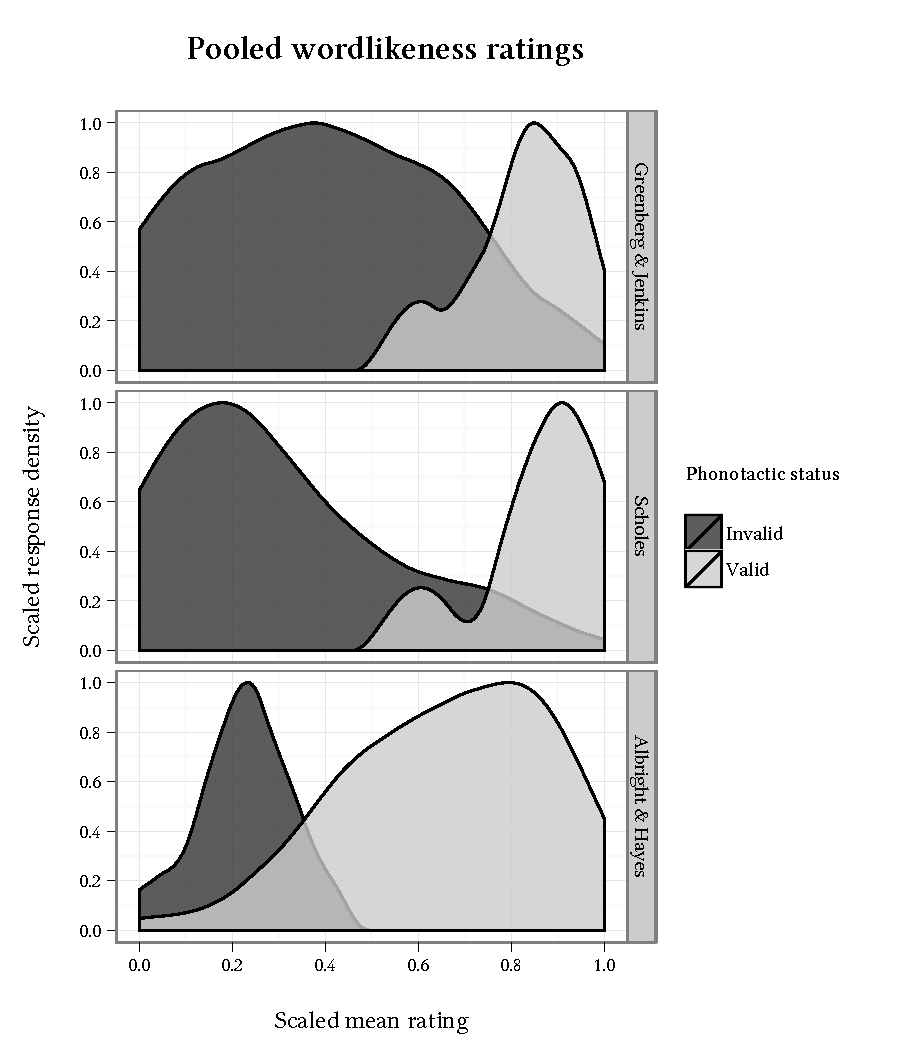
\includegraphics{density.pdf}
\caption{Average ratings of individual nonce words, linearly transformed to the interval [0, 1], tend to clump into two groups with little overlap; words which consist of  attested onsets and rimes receive ratings near ceiling, whereas ratings of phonotactically invalid words are spread across the lower half of the spectrum.}
\end{figure}

\subsubsection{Maximum entropy phonotactics}

\citeauthor{Hayes2008a} (\citeyear{Hayes2008a}; henceforth H\&W) develop a sophisticated model of phonotactic grammaticality which estimates a probability distribution over phoneme sequences by weighing constraints according to the principle of maximum entropy. H\&W find that the predictions of their model are closely correlated with the \citet{Scholes1966} wordlikeness ratings. A direct replication of their predictions was attempted by using the software, model parameters, and training data as described in that study. Since the training of the maximum entropy model is inherently stochastic, producing slightly different outcomes on each run, the lowest scoring of ten runs is reported (H\&W:396), though in general there is not a great deal of variation between individual runs. One limitation of this model is that it is not feasible to score whole words, as the number of constraints which must be inspected grows expontentially as their scope increases. Following H\&W and of \citet{Albright2009a}, who also applies the maximum entropy model to the \citet{Albright2003b} norms, the model is trained and scored only on stimulus onsets. However, as a consequence, the maximum entropy model performs particularly poorly on this data set, as many stimuli contain phonotactic violations in other positions.

\subsubsection{Segment bigram probability}

The bigram probability of a sequence $ijk$ is the product of the probability of an sequence-initial $i$, the probability that $j$ follows $i$, and the probability that $k$ follows $j$, and the product of sequence-final \emph{k}.

\begin{unlabeledexample}
$\displaystyle \hat{p}(ijk) = p(i|\textrm{start}) \cdot p(j|i) \cdot p(k|j) \cdot p(\textrm{stop}|k)$
\end{unlabeledexample}

\noindent Bigram models are widely used in natural language processing, and \citet{Albright2009a} considers their relevance to modeling wordlikeness judgements. While the focus of \citeauthor{Albright2009a}'s study is on developing a model which uses bigrams over phonological features rather than segments themselves, \citeauthor{Albright2009a}'s evaluation, which includes both the \citeauthor{Scholes1966} and \citeauthor{Albright2003b} data sets, finds an advantage for segmental bigrams. 

\citeauthor{Albright2009a} estimates bigram probabilities using the method of maximum likelihood over types in the lexicon. The variant of segmental bigrams used here computes probabilities with a simple type of smoothing in which the count of all possible bigrams (including those never observed) are incremented by one. This technique is known as Laplacian, or ``add one'' smoothing. This has the desirable effect that no nonce word is ever assigned a zero probability, and produces in a small increase in the correlation between the \citeauthor{Albright2003b} wordlikeness norms compared with the maximum likelihood estimate (Table \ref{albrightimproved}). For all three data sets, this model also consistenly outperforms ``positional'' probability models implemented by \citet{Vitevitch2004} and \citet{Vaden2009}, and thus these are not considered further. The bigram model consistently performs well in all the evaluations, and has the highest Spearman correlation with the \citeauthor{Greenberg1964} and \citeauthor{Scholes1966}, and is frequently second place model to the binary baseline elsewhere.

\begin{table} \label{albrightimproved}
\centering
\begin{tabular}{l r r r}
\toprule
                         & maximum likelihood & Laplacian smoothing \\
\midrule
Spearman $\rho$          & 0.660              & \textbf{0.708} \\
Kendall $\tau_b$         & 0.467              & \textbf{0.506} \\
Goodman-Kruskal $\gamma$ & 0.473              & \textbf{0.509} \\
\bottomrule
\end{tabular}
\caption{Laplacian smoothing increases the correlation between the segmental bigram model proposed by \citet{Albright2009a}, which uses maximum likelihood estimation, and the \citet{Albright2003b} wordlikeness norms. All correlations are significant at $p = 0.05$.}
\end{table}

\subsubsection{Neighborhood density}

There are now many methods for computing similarity between nonce words and existing words, long thought to be reflected in wordlikeness judgements. 
For this study, a number of such methods were evaluated, including the Generalized Neighborhood Model \citep{Bailey2001}, PLD20 \citep{Suarez2011}, and a number of variations on neighborhood density \citep{Coltheart1977} provided by \citet{Vaden2009}. The best performance was obtained with the simplest version of neighborhood density, which is defined as the number of real monomorphemic words which can be changed into the target nonce word by a single insertion, deletion, or substitution of a phone. For instance, the neighbors of \emph{blick} include \emph{blink} (insertion), \emph{lick} (deletion) and \emph{black} (substitution). While many studies \citep[e.g.,][]{Bailey2001} report robust lexical similarity effects, it may be that the relatively weak performance of neighborhood density is the result of the presence of gross phonotactic violations.

\subsection{Discussion} \label{2discussion}

\subsubsection{The gradience hypothesis}

The primary result is that no gradient model reliably exceeds the accuracy of the binary baseline. Despite this, there are relatively strong correlations between the binary baseline and these gradient models (see Table \ref{bcor}). However, the fact that the gradient models are generally outperformed by the binary baseline suggest that they do not reliably predict intermediate ratings. To quantify this, the following method was used to estimate the residual contribution of the three gradient models once gross phonotactic violations are taken into account. Instead of calculating rank correlations directly on the model scores as in Table \ref{cor}, the model scores are mapped to ranks with the additional constraint that all ``valid'' stimlui be ranked above all ``invalid'' stimuli. The resulting ranks are used to compute new correlation statistics. Finally, the binary baseline correlation is subtracted from this number, so that the resulting value is the amount of improvement derived from augmenting the binary model with gradience. These difference numbers are shown in Table \ref{controlled}. In most cases, including the gradient models on top of the binary baseline produces a worse correlation than is obtained with the binary baseline alone. The intepretation of this is direct, at least in the case of $\tau_b$ and $\gamma$. Each gradient model draws contrasts within the sets of phonotactically valid and invalid clusters, respectively. For instance, the bigram model favors \emph{troog} [tɹuːg] over \emph{swach} [swætʃ], though neither contains any gross phonotactic violation. Among these contrasts, however, the majority are not reflected in relative wordlikeness judgements. For instance, \emph{troog} is rated less English-like than \emph{swach}. This is stark evidence against the gradience hypothesis.

\begin{table} \label{bcor}
\centering
\begin{tabular}{l r r r}
\toprule
Kendall $\tau_b$          & maxent         & bigram         & density  \\
\midrule
\citealt{Greenberg1964}   & 0.670          & \textbf{0.680} & 0.501 \\
\citealt{Scholes1966}     & \textbf{0.685} & 0.632          & 0.639 \\
\citealt{Albright2003b}   & 0.542          & 0.603          & \textbf{0.623} \\
\bottomrule
\end{tabular}
\caption{The binary baseline is strongly correlated with the three gradient model scores; all correlations are significant at $p = 0.05$.}
\end{table}

\begin{table} \label{controlled}
\centering
\begin{tabular}{l r r r}
\toprule
$\Delta$ Spearman $\rho$          & maxent            & bigram            & density  \\
\midrule
\citealt{Greenberg1964}  & $-0.060$          &  \textbf{0.038} & $-0.017$ \\
\citealt{Scholes1966}    & $-0.029$          &  \textbf{0.047} & $-0.035$ \\
\citealt{Albright2003b}  & $-0.008$          & $-0.015$          & \textbf{0.018} \\
\midrule
$\Delta$ Kendall $\tau_b$         & maxent            & bigram            & density  \\
\midrule
\citealt{Greenberg1964}  & $-0.114$          & \textbf{$-$0.007} & $-0.084$ \\
\citealt{Scholes1966}    & $-0.067$          & \textbf{0.003}  & $-0.061$ \\
\citealt{Albright2003b}  & \textbf{$-$0.038} & $-0.092$          & $-0.049$ \\
\midrule
$\Delta$ Goodman-Kruskal $\gamma$ & maxent            & bigram            & density  \\
\midrule
\citealt{Greenberg1964}  & $-0.268$          & \textbf{$-$0.260} & $-0.337$ \\
\citealt{Scholes1966}    & $-0.361$          & \textbf{$-$0.313} & $-0.345$ \\
\citealt{Albright2003b}  & \textbf{$-$0.137} & $-0.443$          & $-0.386$ \\
\bottomrule
\end{tabular}
\caption{The change in rank correlation generated by augmenting the purely binary model with gradient predictions is small and in most cases it is negative.}
\end{table}

\subsubsection{Possible extensions to the binary baseline}

The strong performance of the binary baseline should not be taken as evidence either that wordlikenesss judgements are binary, or that the binary baseline is a plausible model. The most serious limitation of this evaluation is the primitive nature of the binary baseline. The inability to generalization within onsets and rimes is a serious flaw, as is the assumption of independence of onset and rime. A cognitively plausible version of this model must entertain phonotactic generalizations that are larger than these units.

A possible further extension to the binary baseline would be the introduction of additional levels of wellformedness. While the evaluation has shown that current gradient models do not reliably identify intermediate wellformedness, it does seem possible to identify at least three levels of grammaticality: for instance, one might share the intuition that \emph{zhlick} [ʒlɪk] is more similar to English than \emph{bnick}, though both have unattested onsets. 

There are precedents for labeling certain attested words as phonotactically ``peripheral'' (see, e.g., the appendices in \citealt{Myers1987} and \citealt{Borowsky1989}); such words are regarded as lexical exceptions to language-general principles of syllabification. If this extends to nonce words, then an intermediate level of grammaticality could be assigned to ``possible'' but formally marked words. Another likely source of additional levels of grammaticality is the cumulative effect of multiple phonotactic violations. While, as \citet{Coleman1997} note, classic model predict taht a nonce word is as ill-formed as its worst deviation from syllable structure, 
it is possible to imagine that multiple phonotactic violations would result in greater degrees of ill-formedness. Many competing models make this prediction (e.g., \citealt{Legendre1990}, \citealt{Levelt2000}, \citealt{Goldwater2003}, \citealt{Jager2007}, \citealt{Albright2008}, \citealt{Pater2009b}) but despite this, there is currently no data bearing on whether cumulative effects are found in wordlikeness tasks.

\section{Conclusion}

This chapter has evaluated the axiom of gradience as a falsifiable alternative hypothesis. The surprising result is that virtually all of the apparent coverage of state-of-the-art gradient phonotactic models is simply a reflection of their ability to distinguish between the possible and the totally impossible; beyond this, they are unreliable. A trivial baseline, endowed with few abilities to project beyond the observed data, generally outperforms the state of the art. It follows that the projections made by the state-of-the-art gradient models are not like those made by speakers.

%\subsection{Future directions}
%\subsubsection{Interspeaker variation}
%The studies analyzed above all use ratings averaged across subjects. While aggregation of this type is quite common in psycholinguistics, it is undesirable as a statistical practice: it drastically increases the chance of a Type II error, the error of failing to reject a null hypothesis when the null hypothesis is false \citep[][8f.]{Baayen2004}. Further, little is known about intraspeaker variation in wordlikeness judgements and even less about intraspeaker variation, but \citet{Shademan2007} does find suggestive differences between older and younger adults. It would be extremely interesting to correlate differences in speakers with external factors like age, level of education, and exposure to foreign languages. 
%\subsubsection{Mixed modalities}
%While the use of auditory stimulus presentation seems preferable to rating orthographic words, the possibiltiy of misperception introduces a potential confound. \citet{Scholes1966} mentions that a few of his stimuli were frequently misperceived, and a number of studies \citep{Massaro1983,Halle1998b,Pitt1998,Dupoux1999,Berent2007a,Davidson2007} uncover positive correlations between phonotactic acceptability and accurate perception. If the phonotactically invalid cluster in *\emph{srest} is perceived as a phonotactically valid cluster with similar acoustic features, such as [ʃr], it will likely receive an inflated wordlikeness rating. In many psycholinguistic tasks, the behavioral measure of interest comes with a validation of correct perception: for instance, in shadowing tasks, reaction times are the primary behavioral measure but shadowing errors are also informative behavioral measures \citep[e.g.,][]{Marslen-Wilson1978}. Wordlikeness studies could combine transcription or repetition tasks with judgement tasks to confirm correct perception and perhaps to enhance the online nature of the task.
%Several recent studies have investigated the role of phonotactics using an auditory lexical decision tasks \citep[e.g.,][]{Berent2001a,Berent2004,Shatzman2007a}. A recent study by \citet{Coetzee2008b} is particularly relevant to the larger questions of this dissertation, though the results are ultimately inconclusive. \citeauthor{Coetzee2008b} claims that words of the form [spVp, skVk] (e.g., *\emph{spep} [spɛp], *\emph{skeek} [skiːk]) are impossible in English, whereas [stVt] words (e.g., *\emph{stoit} [stɔɪt]) are wellformed. In addition to a traditional wordlikeness task, \citet{Coetzee2008b} includes stimuli of this type in a lexical decision task, under the hypothesis that the illformed nonce words, those of the shape [spVp, skVk], will be more quickly rejected than valid [stVt] stimuli, a prediction which is borne out. However, there is no need to provide a phonotactic interpretation of these effects. It is known that auditory tasks reaction times are significantly slower for non-words with dense cohorts, that is, nonce words like *\emph{hup} [hʌp] which share initial segments with many real words (e.g., \emph{hull}, \emph{hut}, etc.). These effects are found across modalities \citep[e.g.,][]{Marslen-Wilson1978,Marslen-Wilson1984} and appear to be particularly attentuated for non-word onsets \citep{Cole1980,Vitevitch2002}. Since [st] onsets are far more frequent than [sp] or [sk] onsets \citep[][395]{Hayes2008a}, this alone could explain the variation in reaction times. Despite this, nonce word lexical decision with controls for lexical cohort effects shows potential as a substitute for wordlikeness judgements in phonotactics research. 
%\subsubsection{Data availability}
%There are still very few publicly available wordlikeness databases, and several authors who were contacted for this project declined to share data. Not only does this make large-scale model comparison difficult, it also means that most wordlikeness studies cannot be replicated except at the conceptual level. Lexical decision researchers now have databases of response times for American \citep{ELP} and British English \citep{BLP}, Dutch \citep{DLP}, French \citep{FLP}, and Malay \citep{MLP}. Given the simplicity of wordlikeness judgements (a sort of linguistic \emph{Drosophilia}), the time for a publicly available ``English Wordlikeness Project'' has come.
%\subsubsection{Non-parametric statistics}
%The surprising results of this evaluation can be traced directly to two methodological improvements which should be more widely adopted. First, model comparison studies must replace parametric statistical models, such as Pearson correlation, with non-parametric equivalents. Given the tendency of ratings to cluster at endpoints, Pearson correlations are inflated \citep[][23, fn. 12]{Albright2009a} and the assumptions of the test are flagrantly violated. A shift towards non-parametric comparison appears to be well underway: \citet{Hayes2008a} also report model correlations using the Spearman $\rho$ and \citet{Albright2009a} focuses on a variant of the Kendall correlation called $tau_c$. %On the other hand, both \citeauthor{Hayes2008a} and \citeauthor{Albright2009a} ultimately use parametric statistics for model comparison.
%\begin{table}
%\centering
%\begin{tabular}
%\toprule
%                        & accuracy & precision & recall & F$_1$ & MCC   \\
%\midrule
%\citealt{Greenberg1964} & 0.846    & 1.000     & 0.800  & 0.889 & 0.693 \\
%\citealt{Scholes1966}   & 0.952    & 0.947     & 0.900  & 0.923 & 0.889 \\
%\citealt{Albright2003b} & 0.920    & 0.938     & 0.953  & 0.946 & 0.797 \\
%\bottomrule
%\end{tabular}
%\end{table}
% EM \citet{EM} 
%\begin{table}
%\centering
%\begin{tabular}{l | r r}
%\toprule
%                        & $\chi^2_{3}$ & $p$-value  \\
%\midrule
%\citealt{Greenberg1964} &  5.190       & 0.158      \\
%\citealt{Scholes1966}   & 48.964       & 1.3\e{-15} \\
%\citealt{Albright2003b} & 16.186       & 0.001      \\
%\bottomrule
%\end{tabular}
%\caption{This is my caption}
%\end{table}
%\footnote{This is conceptually similar to the technique of residualization discussed by \citet{Gorman2010c}.}
%\begin{unlabeledexample}
%$\displaystyle P = s^{1/7.4}$
%\end{unlabeledexample}
%\noindent Even then, \citet[][23, fn. 12]{Albright2009a} 
%An interesting feature of this data set is that includes a diverse set of onsets ranging from frequent to impossible, but only a few common rimes; \citet{Albright2009a} speculates this might have made the onsets more salient to the subjects than tehy would be otherwise.
%The Pearson correlation depends on an interval assumption, which holds that the difference between, for example, ``1. completely bi disagree'' and ``2. agree'' is in some sense identical to that between ``3. neither agree nor disagree'' and ``4. agree''. \citet{Stevens1946} already observes that there is no a priori basis for this assumption, and similar objections can be leveled for other rating methods. Secondly, 
%the Pearson correlation assumes a linear relationship between model scores and ratings; when this assumption is violated, researchers must search for a satisfactory transformation to produce linearity. 
%As \citet{Halle1962} argues, this eliminates the need for additional grammatical machinery.
%\begin{quote}
%\ldots{}we are forced to incorporate into every complete generative grammar a characterization of the distinction between admissible and inadmissible segment sequences. The fact effectively cuts the ground out from under the recent suggestion that generative grammars be supplemented with special phonological grammars\ldots{} \citep[][61]{Halle1962}
%\end{quote}
